\documentclass[
	classe=$2^{de}$
]{évaluation}

\usepackage{tcolorbox}
\usepackage{tikz-repère}
\usepackage{tkz-tab}

% First one is correct
\newcommand{\correctionStrike}[2]{%
\ifdefined\makeCorrection%
\sout{#1}/#2
\else%
#1/#2
\fi%
}

\renewcommand{\correctionDots}[1]{\correctionOr{{\color{red}#1}}{....................}}

\date{5 mai 2023}

\newcommand{\makeCorrection}{}
\begin{document}

\title{Évaluation : fonctions (sujet A)}
\maketitle

\begin{exercice}
	On dispose d'une fonction $f$, telle que
	\begin{align*}
		f(-1) & = 2 & f(0) & = 1 & f(1) & = 6 & f(2) & = 2 & f(3) & = -1 & f(4) & = 6
	\end{align*}
	Remplir :
	\begin{multicols}{2}
		\begin{itemize}
			\item[] $-1$ est \correctionDots{un antécédent} de $2$
			\item[] $-1$ est \correctionDots{l'image} de $3$
			\item[] \correctionDots{$1$ et $4$} sont les antécédents de $6$
			\item[] \correctionDots{$6$} est l'image de $1$
		\end{itemize}
	\end{multicols}
\end{exercice}

\begin{exercice}
	\begin{enumerate}
		\item Si $f(x) = x - 3$,

		      $f(4) = 4 - 3 = \circled{1}$
		\item Si $f(x) = \dfrac{5x + 1}{x - 3}$,

		      $f(-1) = \dfrac{5×(-1) + 1}{-1 - 3} = \dfrac{-4}{-4} = \circled{1}$
		\item Si $f(x) = x^3 - x^2$,

		      $f(7) = 7^3 - 7^2 = 343 - 49 = \circled{294}$.
	\end{enumerate}
\end{exercice}

\begin{exercice}
	\pgfmathsetmacro\scale{0.7}
	\begin{multicols}{2}
		\begin{center}
			\begin{tikzpicture}[scale=\scale]
				\tikzRepere{-3.5}{3.5}{-2.5}{2.5}
				\draw[domain=-4:4,thick,blue] plot({\x},{0.5*\x+1});
			\end{tikzpicture}
			$$ f(x) = \correctionDots{\dfrac{1}{2}x + 1} \hspace{2em} f(100) = \correctionDots{51} $$
		\end{center}

		\begin{center}
			\begin{tikzpicture}[scale=\scale]
				\tikzRepere{-3.5}{3.5}{-2.5}{2.5}
				\draw[domain=-1.5:1.5,thick,blue] plot({\x},{2*\x});
			\end{tikzpicture}
			$$ g(x) = \correctionDots{2x} \hspace{2em} g(100) = \correctionDots{200} $$
		\end{center}

		\columnbreak

		\begin{center}
			\begin{tikzpicture}[scale=\scale]
				\tikzRepere{-3.5}{3.5}{-2.5}{2.5}
				\draw[domain=-2:1,thick,blue] plot({\x},{-2*\x-1});
			\end{tikzpicture}
			$$ h(x) = \correctionDots{-2x - 1} \hspace{2em} h(100) = \correctionDots{-201} $$
		\end{center}

		\begin{center}
			\begin{tikzpicture}[scale=\scale]
				\tikzRepere{-3.5}{3.5}{-2.5}{2.5}
				\draw[domain=-1:4,thick,blue] plot({\x},{\x-2});
			\end{tikzpicture}
			$$ i(x) = \correctionDots{x - 2} \hspace{2em} i(100) = \correctionDots{98} $$
		\end{center}

	\end{multicols}
\end{exercice}

\newpage

\begin{exercice}
	\begin{enumerate}
		\item Le domaine de définition de $f$ est $\intervalle{[}{-4}{4}{]}$.
		\item
		      \begin{enumerate}
			      \item L'image de $-4$ par $f$ est $-1$.
			      \item Les antécédents de $1$ par $f$ sont $-2$ et $4$.
			      \item la valeur de $f(2)$ est $-2$.
		      \end{enumerate}
		\item \
		      \begin{center}
			      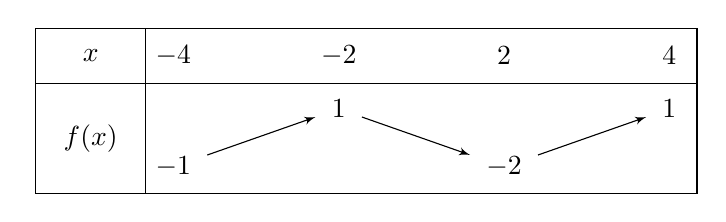
\begin{tikzpicture}[scale=0.7]
				      \tkzTabInit{$x$ / 1 , $f(x)$ / 2}{$-4$, $-2$, $2$, $4$}
				      \tkzTabVar{-/ $-1$, +/ $1$, -/ $-2$, +/ $1$}
			      \end{tikzpicture}
		      \end{center}
	\end{enumerate}
\end{exercice}

\begin{exercice}
	\begin{enumerate}
		\item D'après l'énoncé, la hauteur de la balle en l'abscisse $0$ est $50$cm. On a donc $f(0) = 50$.
		\item D'après la question $1$, on a l'égalité $f(0) = 50$, soit $-\dfrac{1}{40}×0^2 + 2×0 + a = a = 50$.
		\item \

		      \begin{center}
			      \begin{tikzpicture}[scale=0.9]
				      \pgfmathsetmacro\scale{10}
				      \tikzRepere{0}{11}{0}{10}[\scale][\scale][abscisse (cm)][hauteur (cm)]

				      \ifdefined\makeCorrection
					      \draw[domain=0:10,very thick,red] plot({\x},{(-0.025*\x*\x*\scale*\scale + 2*\x*\scale + 50)/\scale});
				      \fi
			      \end{tikzpicture}
		      \end{center}
		\item \

		      \begin{center}
			      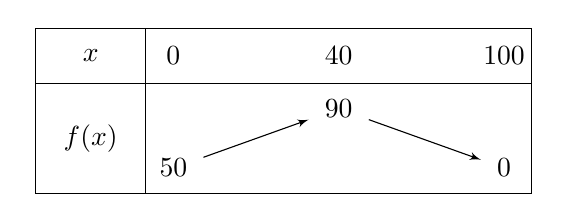
\begin{tikzpicture}[scale=0.7]
				      \tkzTabInit{$x$ / 1 , $f(x)$ / 2}{$0$, $40$, $100$}
				      \tkzTabVar{-/ $50$, +/ $90$, -/ $0$}
			      \end{tikzpicture}
		      \end{center}
		\item
		      \begin{enumerate}
			      \item La hauteur maximale atteinte par la balle est $90$cm.
			      \item La balle est retombée sur le sol à l'abscisse $100$cm.
		      \end{enumerate}
	\end{enumerate}
\end{exercice}

%===========================================
%================ SUJET B ==================
%===========================================

\newpage\setcounter{exercice}{1}

\title{Évaluation : fonctions (sujet B)}
\maketitle

\begin{exercice}
	On dispose d'une fonction $f$, telle que
	\begin{align*}
		f(-2) & = 2 & f(-1) & = 1 & f(0) & = 6 & f(1) & = 2 & f(2) & = -1 & f(3) & = 6
	\end{align*}
	Remplir :
	\begin{multicols}{2}
		\begin{itemize}
			\item[] $-1$ est \correctionDots{un antécédent} de $1$
			\item[] $-1$ est \correctionDots{l'image} de $2$
			\item[] \correctionDots{$0$ et $3$} sont les antécédents de $6$
			\item[] \correctionDots{$2$} est l'image de $1$
		\end{itemize}
	\end{multicols}
\end{exercice}

\begin{exercice}
	\begin{enumerate}
		\item Si $f(x) = x - 2$,

		      $f(3) = 3 - 2 = \circled{1}$.
		\item Si $f(x) = \dfrac{3x + 1}{x + 2}$,

		      $f(-1) = \dfrac{3×(-1) + 1}{-1 + 2} = \dfrac{-2}{1} = \circled{-2}$
		\item Si $f(x) = x^3 - x^2$,

		      $f(5) = 5^3 - 5^2 = \circled{100}$.
	\end{enumerate}
\end{exercice}

\begin{exercice}
	\pgfmathsetmacro\scale{0.7}
	\begin{multicols}{2}
		\begin{center}
			\begin{tikzpicture}[scale=\scale]
				\tikzRepere{-3.5}{3.5}{-2.5}{2.5}
				\draw[domain=-1.5:1.5,thick,blue] plot({\x},{2*\x});
			\end{tikzpicture}
			$$ f(x) = \correctionDots{2x} \hspace{2em} f(100) = \correctionDots{200} $$
		\end{center}

		\begin{center}
			\begin{tikzpicture}[scale=\scale]
				\tikzRepere{-3.5}{3.5}{-2.5}{2.5}
				\draw[domain=-4:4,thick,blue] plot({\x},{0.5*\x+1});
			\end{tikzpicture}
			$$ g(x) = \correctionDots{\dfrac{1}{2}x + 1} \hspace{2em} g(100) = \correctionDots{51} $$
		\end{center}

		\columnbreak

		\begin{center}
			\begin{tikzpicture}[scale=\scale]
				\tikzRepere{-3.5}{3.5}{-2.5}{2.5}
				\draw[domain=-1:4,thick,blue] plot({\x},{\x-2});
			\end{tikzpicture}
			$$ h(x) = \correctionDots{x - 2} \hspace{2em} h(100) = \correctionDots{98} $$
		\end{center}

		\begin{center}
			\begin{tikzpicture}[scale=\scale]
				\tikzRepere{-3.5}{3.5}{-2.5}{2.5}
				\draw[domain=-2:1,thick,blue] plot({\x},{-2*\x-1});
			\end{tikzpicture}
			$$ i(x) = \correctionDots{-2x - 1} \hspace{2em} i(100) = \correctionDots{-201} $$
		\end{center}
	\end{multicols}
\end{exercice}

\newpage

\begin{exercice}
	\begin{center}
		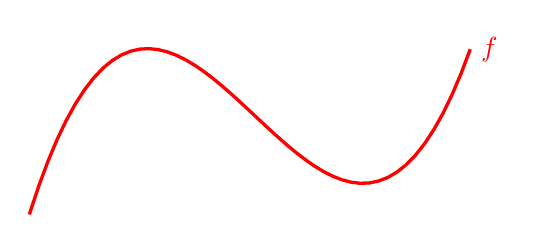
\begin{tikzpicture}[scale=0.7]
			\tikzRepere{-4.5}{4.5}{-2.5}{1.5}
			\draw[domain=-4:0,very thick,red] plot({\x},{1/9*(0.7375*\x*\x*\x - 0.2125*\x*\x - 8.425*\x - 1.1)});
			\draw[domain=0:4,very thick,red] plot({\x},{1/9*(0.7375*\x*\x*\x - 0.2125*\x*\x - 8.425*\x - 1.1)}) node[right] {$f$};
		\end{tikzpicture}
	\end{center}

	\begin{enumerate}
		\item Le domaine de définition de $f$ est $\intervalle{[}{-4}{4}{]}$.
		\item
		      \begin{enumerate}
			      \item L'image de $-4$ par $f$ est $-2$.
			      \item Les antécédents de $1$ par $f$ sont $-2$ et $4$.
			      \item la valeur de $f(1)$ est $-1$.
		      \end{enumerate}
		\item \

		      \begin{center}
			      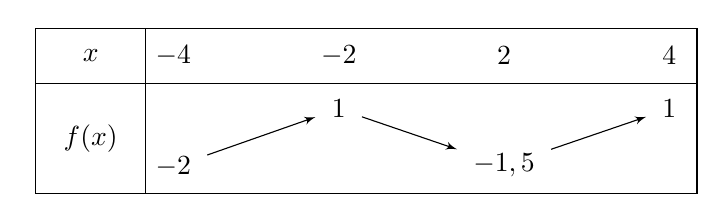
\begin{tikzpicture}[scale=0.7]
				      \tkzTabInit{$x$ / 1 , $f(x)$ / 2}{$-4$, $-2$, $2$, $4$}
				      \tkzTabVar{-/ $-2$, +/ $1$, -/ ${-1,5}$, +/ $1$}
			      \end{tikzpicture}
		      \end{center}
	\end{enumerate}
\end{exercice}

\begin{exercice}
	\begin{enumerate}
		\item La hauteur de la balle en l'abscisse $0$ est $48$cm. On a alors $f(0) = 48$.
		\item D'après la question $1$, on a l'égalité $f(0) = 48$, soit $-\dfrac{1}{50}×0^2 + 2×0 + a = a = 48$.
		\item \

		      \begin{center}
			      \begin{tikzpicture}[scale=0.85]
				      \pgfmathsetmacro\scale{10}
				      \tikzRepere{0}{13}{0}{10}[\scale][\scale][abscisse (cm)][hauteur (cm)]

				      \ifdefined\makeCorrection
					      \draw[domain=0:12,very thick,red] plot({\x},{(-1/50*\x*\x*\scale*\scale + 2*\x*\scale + 48)/\scale});
				      \fi
			      \end{tikzpicture}
		      \end{center}
		\item \

		      \begin{center}
			      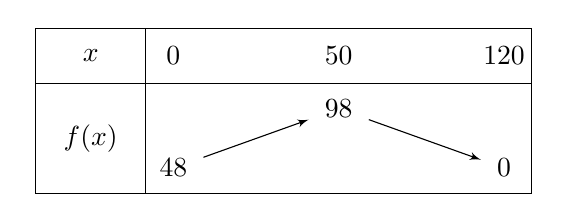
\begin{tikzpicture}[scale=0.7]
				      \tkzTabInit{$x$ / 1 , $f(x)$ / 2}{$0$, $50$, $120$}
				      \tkzTabVar{-/ $48$, +/ $98$, -/ $0$}
			      \end{tikzpicture}
		      \end{center}
		\item
		      \begin{enumerate}
			      \item La hauteur maximale atteinte par la balle est $98$cm.
			      \item La balle est retombée sur le sol à l'abscisse $120$cm.
		      \end{enumerate}
	\end{enumerate}
\end{exercice}

\end{document}